\documentclass[10 pt,usenames,dvipsnames, oneside]{article}
\usepackage{../../../modelo-ensino-medio}



\begin{document}

\begin{center}
  \begin{minipage}[l]{3cm}

\includegraphics[width=2cm]{logo}    
\end{minipage}\hfill
\begin{minipage}[r]{.8\textwidth}
 {\Large \scshape Atividade: Indo para escola}  
\end{minipage}
\end{center}
\vspace{.2cm}

\ifdefined\prof
\begin{objetivos}
\item \textbf{LAF1} Compreender função como uma relação de dependência entre duas variáveis, as ideias de domínio, contradomínio e imagem, e suas representações algébricas e gráficas e utilizá-las para analisar, interpretar e resolver problemas em contextos diversos, inclusive fenômenos naturais, sociais e de outras áreas.
\end{objetivos}

\begin{goals}
\begin{enumerate}

\item[OE1] Fazer uso de simbologia matemática para representar informações apresentadas pictórica e verbalmente.

\item[OE2] Interpretar e relacionar informações a partir da representação gráfica apresentada.

\end{enumerate}

\tcblower

\begin{itemize}
\item É importante que os estudantes percebam o significado de dois pontos estarem na mesma horizontal ou na mesma vertical.

\item Chame a atenção para o uso da escala.
\end{itemize}

\end{goals}

\bigskip
\begin{center}
{\large \scshape Atividade}
\end{center}
\fi

Arthur, Caetano, Gael, Levi e Pedro utilizam a mesma avenida para ir à escola a cada manhã. Levi vai com seu pai de carro, Arthur de bicicleta e Gael caminhando. Os demais variam, a cada dia, a forma como percorrem o trajeto. O mapa a seguir mostra a posição da casa de cada um em relação à escola.
\phantomsection\label{\detokenize{AF106-5:fig-mapa-escola}}

\begin{figure}[H]
\centering

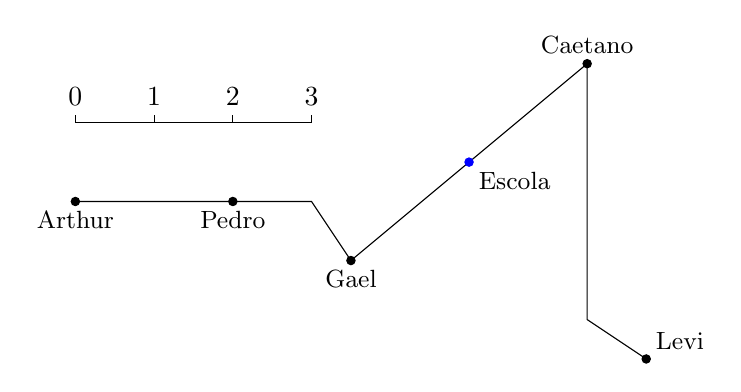
\begin{tikzpicture}
\tikzstyle{ponto}=[circle, minimum size=3pt, inner sep=0, draw=black, fill=black, shift only]
\draw(-2,2)grid(1,2.1);
\foreach \x in {0,1,2,3}
\node at (\x - 2,2.1)[above]{\x};
\coordinate (A) at (-2,1);
\coordinate (B) at (0,1);
\coordinate (C) at (1,1);
\coordinate (D) at (1.5,.25);
\coordinate (E) at (3,1.5);
\coordinate (F) at (4.5,2.75);
\coordinate (G) at (4.5,-.5);
\coordinate (H) at (5.25,-1);
\draw(A)--(B)--(C)--(D)--(E)--(F)--(G)--(H);
\node[ponto] at (A){};\node[ponto] at (B){};\node[ponto] at (D){};\node[ponto, blue] at (E){};\node[ponto] at (F){};\node[ponto] at (H){};
\node[below] at (A){\small Arthur};\node[below] at (B){\small Pedro };\node[below] at (D){\small Gael};\node[below right] at (E){\small Escola};\node[above] at (F){\small Caetano};\node[above right] at (H){\small Levi};
\end{tikzpicture}
\end{figure}

Os pontos marcados no plano cartesiano abaixo fornecem informações sobre a jornada de cada criança na última segunda-feira.
\phantomsection\label{\detokenize{AF106-5:fig-grafico-jornada}}

\begin{figure}[H]
\centering

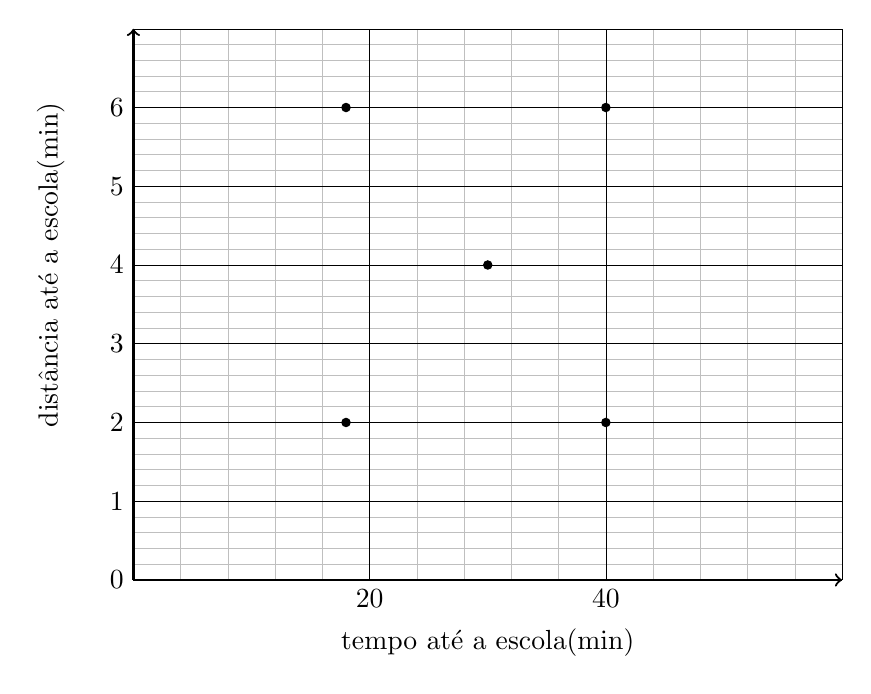
\begin{tikzpicture}
\tikzstyle{ponto}=[circle, minimum size=3pt, inner sep=0, draw=black, fill=black, shift only]
\begin{scope}[xscale=3]
\draw[help lines,xstep=.2,ystep=.2, lightgray] (0,0) grid (3,7);
\draw[help lines, black, xstep=1, ystep=1] (0,0) grid (3,7);
\draw[thick,->](0,0)--(3,0);
\draw[thick,->](0,0)--(0,7);
\draw(1.5,-.8)node{ tempo até a escola(min)};
\draw(-.35,4)node[rotate=90]{distância até a escola(min)};
\node[ponto] at(.9,2){};
\node[ponto] at(.9,6){};
\node[ponto] at(1.5,4){};
\node[ponto] at(2,2){};
\node[ponto] at(2,6){};
\foreach \y in {0,1, 2, 3, 4, 5, 6}
\draw(0,\y) [left] node {\y};
\draw(1,0)node[below]{20};
\draw(2,0)node[below]{40};
\end{scope}
\end{tikzpicture}
\end{figure}

\begin{enumerate}
\item {} 
Associe cada ponto do gráfico com o nome da criança que ele representa.

\item {} 
Como Pedro e Caetano foram para a escola na última segunda-feira? Por que?

\end{enumerate}

{\color{red}\bfseries{}{}`}\emph{{}`Adaptado de *The Language of Functions and Graphs}, Shell Centre for Mathematical Education Publications Ltd., 1985.


\ifdefined\prof

\begin{solucao}
\begin{enumerate}

\item\adjustbox{valign=t}{\begin{minipage}{\linewidth}
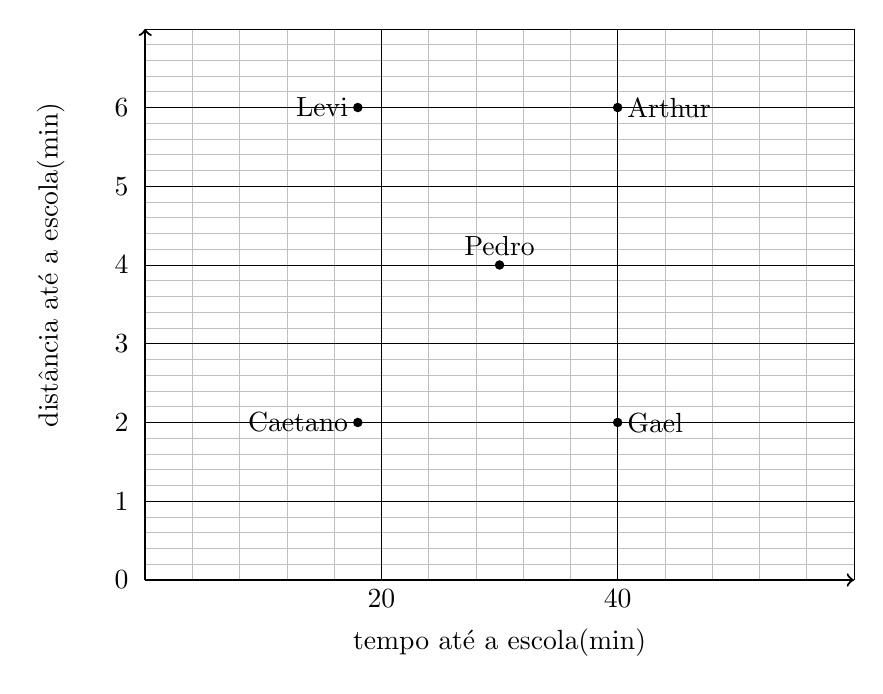
\begin{tikzpicture}
\tikzstyle{ponto}=[circle, minimum size=3pt, inner sep=0, draw=black, fill=black, shift only]
\begin{scope}[xscale=3, every node/.style={black}, every path/.style={black}]
\draw[help lines,xstep=.2,ystep=.2, lightgray] (0,0) grid (3,7);
\draw[help lines, black, xstep=1, ystep=1] (0,0) grid (3,7);
\draw[thick,->](0,0)--(3,0);
\draw[thick,->](0,0)--(0,7);
\draw(1.5,-.8)node{tempo até a escola(min)};
\draw(-.4,4)node[rotate=90]{distância até a escola(min)};
\node[ponto] at(.9,2){};
\node[ponto] at(.9,6){};
\node[ponto] at(1.5,4){};
\node[ponto] at(2,2){};
\node[ponto] at(2,6){};
\node[  left] at(.9,2){Caetano};
\node[left] at(.9,6){ Levi};
\node[above] at(1.5,4){Pedro};
\node[right] at(2,2){Gael};
\node[right] at(2,6){Arthur};
\foreach \y in{0,1, 2, 3, 4, 5, 6}
\draw(-.1,\y)node{\y};
\draw(1,0)node[below]{20};
\draw(2,0)node[below]{40};
\end{scope}
\end{tikzpicture}
\end{minipage}}

\item Pedro e Caetano foram para a escola de bicicleta ou correndo (ou de alguma forma que seja mais rápida do que ir a pé e mais lenta que ir de carro). Caetano e Gael moram ambos a $2$ km doa escola. Como Gael, que foi caminhando, levou $40$ minutos, Caetano que gastou aproximadamente $18$ minutos não pode ter ido caminhando. Caetano também não pode ter ido de carro, pois Levi que mora a $6$ km da escola demorou o mesmo tempo que ele e foi de carro.

\end{enumerate}
\end{solucao}
\fi

\end{document}